%%%%%%%%%%%%%%
% LECTURE 18 %
%%%%%%%%%%%%%%

\vspace{1cm}
\noindent\lecture{18}{10/12/2021}
\vspace{0.5cm}

\noindent Abbiamo visto come la CQED\footnote{Abbreviazione per Cavity Quantum Electrodynamics.} modellizzi l'interazione tra un qubit e il campo elettromagnetico quantizzato generato all'interno di una cavità o un risonatore. L'hamiltoniana di Jaynes-Cummings \eqref{eq:ham-jaynes-cummings} fu studiata per la prima volta nel contesto dell'ottica quantistica: non appare solo in questo caso particolare, ma in tutti quei casi in cui un qubit interagisce con uno dei modi quantizzati del campo elettromagnetico, ossia descrive tutte quelle interazioni della forma $\vec d \cdot \vec E$, $\vec \mu \cdot \vec B$, ecc.

\noindent Giunti a questo punto vogliamo discutere il significato fisico che si trova dietro a questa hamiltoniana, in particolare vedremo qualche semplice esempio di codifica di un qubit in un modello CQED. Innanzitutto notiamo che l'hamiltoniana originale non approssimata della relazione \eqref{H_da_riscrivere_4} non poteva essere risolta esattamente, tuttavia grazie alla RWA può essere invece diagonalizzata! 

\noindent Dal punto di vista della QM, l'hamiltoniana \eqref{eq:ham-jaynes-cummings} costituisce un semplice problema di accoppiamento tra spin e oscillatore armonico (le eccitazioni di questo oscillatore sono fotoni). Lo spazio di Hilbert totale è infinito dimensionale in quanto è frutto del prodotto $\mathcal{H}_c \otimes \mathcal{H}_q$, dove $\dim \mathcal{H}_c = \infty$ (infiniti oscillatori). Nonostante ciò, l'hamiltoniana sopra è diagonalizzabile perché è una matrice diagonale a blocchi; per tale ragione suddividiamo gli stati utilizzando la seguente notazione:
\begin{align*}
    &\ket{0} \equiv \ket{g} &\Rightarrow& &&\text{Stato fondamentale del qubit.} \\
    &\ket{1} \equiv \ket{e} &\Rightarrow& &&\text{Stato eccitato del qubit.} \\
    &\ket{n} = \ket{0}, \ket{1}, \ket{2}, \ldots &\Rightarrow& &&\text{Numero di fotoni campo elettromagnetico.}
\end{align*}
La struttura a blocchi è evidente notando che $\ket{e,n} \leftrightarrow \ket{g,n+1}$, ossia sono trasformati l'uno nell'altro dai termini dell'interazione: infatti
\begin{align*}
    \hat a^\dagger \hat \sigma_+ \ket{e,n} &= \sqrt{n+1} \ket{g,n+1} \, , \\
    \hat a \hat \sigma_- \ket{g, n+1} &= \sqrt{n+1} \ket{e,n} \, ,
\end{align*}
perché nel primo caso diseccitiamo lo stato del qubit e creiamo un fotone di diseccitazione (lo stato finale è lo stato fondamentale con un fotone in più), mentre nel secondo caso distruggiamo un fotone della cavità, il quale viene assorbito dallo stato fondamentale, che sarà poi eccitato. Alla luce di questa osservazione possiamo suddividere lo spazio di Hilbert totale $\mathcal{H}$ in
\begin{equation}\label{CQED_states}
    \left\{\ket{g,0}\right\} \, , \quad \left\{ \ket{e,n}, \, \ket{g,n+1}\right\} \, ;
\end{equation}
decomponendo $\mathcal{H}$ in questo modo, ogni qualvolta che si agisce con i termini di interazione in \eqref{eq:ham-jaynes-cummings} si rimane sempre nello stesso sottospazio. Tenendo presente che $\hat{H}_0$ è diagonale, mentre $\hat{H}_I$ è off-diagonal, allora in forma matriciale l'hamiltoniana diventa
\begin{equation*}
    \hat H = \frac 12 \omega_c \mathbb{I} + 
    \begin{pmatrix}
        -\frac{\omega_q}2 & & & \\
        & \begin{pmatrix}
            \omega_c - \frac{\omega_q}2 & g \\
            g & \frac{\omega_q}2
          \end{pmatrix} & & \\
        & & \ddots & \\
        & & & \begin{pmatrix}
            \omega_c(n+1) - \frac{\omega_q}2 & g\sqrt{n+1} \\
            g\sqrt{n+1} & \omega_c n + \frac{\omega_q}2
        \end{pmatrix} \\
    \end{pmatrix}
    \begin{matrix}
        \ket{g,0}\\
        \ket{g,1}\\
        \ket{e,0}\\
        \\
        \ket{g,n+1}\\
        \ket{e,n}
    \end{matrix}\, ,
\end{equation*}
dove il termine iniziale rappresenta l'energia di punto zero, detta \textbf{ZPE} ("Zero Point Energy"). (Gli stati a destra sono per ricordare ciò a cui fanno riferimento i blocchi di questa matrice). Ricordando che il \textbf{detuning} è definito come $\Delta=\omega_q - \omega_c$ e tenendo conto della ZPE, possiamo allora riscrivere il blocco generico (ultimo elemento) della matrice precedente come
\begin{equation*}
    \begin{pmatrix}
        (n+1)\omega_c - \frac{\Delta}2 & \sqrt{n+1}g \\
        \sqrt{n+1}g & (n+1)\omega_c + \frac{\Delta}2
    \end{pmatrix} \, ;
\end{equation*}
diagonalizzando questo blocco, lo spettro dell'hamiltoniana è dato dai seguenti autovalori e autostati
\begin{align*}
    E_+ &= (n+1)\omega_c + \frac 12 \sqrt{\Delta^2+4g^2(n+1)} \, , &\ket{n_+} &= \sin\theta_n \ket{g,n+1} + \cos\theta_n\ket{e,n} \, , \\
    E_- &= (n+1)\omega_c - \frac 12 \sqrt{\Delta^2+4g^2(n+1)} \, , &\ket{n_-} &= \cos\theta_n\ket{g,n+1}-\sin\theta_n\ket{e,n} \, ;
\end{align*} 
ad essi si aggiunge il singolo stato $\ket{g,0}$ con energia $E_0 = - \frac{\Delta}{2}$. Gli stati $\ket{n_-}$ e $\ket{n_+}$ prendono il nome di \textbf{dressed states} e l'angolo $\theta_n$ risulta essere definito come
\begin{equation*}
    \tan {2 \theta_n} = \frac{2g\sqrt{n+1}}{\Delta} \, .
\end{equation*}

\noindent Che cosa succede ad un sistema come questo? L'evoluzione temporale, che ricordiamo essere data da $e^{-i\hat H t}$ (hamiltoniana indipendente dal tempo), realizza delle \textbf{oscillazioni di Rabi} sulla coppia dei \textbf{dressed states}: ogni stato si comporta come un sistema a due livelli che oscilla coerentemente in cicli di assorbimento ed emissione di fotoni in maniera tale che gli stati in \eqref{CQED_states} si trasformino continuamente l'uno nell'altro, ossia $\ket{g,n+1} \leftrightarrow \ket{e,n}$. Confrontando con il caso dei campi esterni, qui abbiamo due accoppiamenti: l'interazione è quantificata da $g$, la forza dell'accoppiamento tra i due sistemi, alla quale si aggiunge però $n$, ovvero il numero dei fotoni. La frequenza di Rabi delle oscillazioni risulta quindi essere data da $\sqrt{\Delta^2+4g^2(n+1)}$: maggiore è il numero di fotoni, più grande sarà la frequenza di oscillazione del qubit.

\noindent In ottica quantistica si è spesso interessati a guardare a situazioni in cui si ha una sovrapposizione di differenti stati con numero di fotoni fissato. In questi contesti l'oscillazione generale è più complicata: ogni insieme di fotoni si accoppia in blocchi di 2 cosicché ogni blocco oscilli a coppie. Il punto fondamentale è che la sovrapposizione di oscillazioni crea una situazione in cui non ci sono oscillazioni! Talvolta è possibile aspettare del tempo a sufficienza fino a quando si ritorna ad osservare un pattern di oscillazioni: tipicamente, quando si sovrappongono molti sistemi oscillatori, si ha interferenza, quindi se si aspetta un tempo sufficiente si possono di nuovo osservare delle oscillazioni (rilevate sperimentalmente).   

\begin{figure}[!ht]
    \centering
    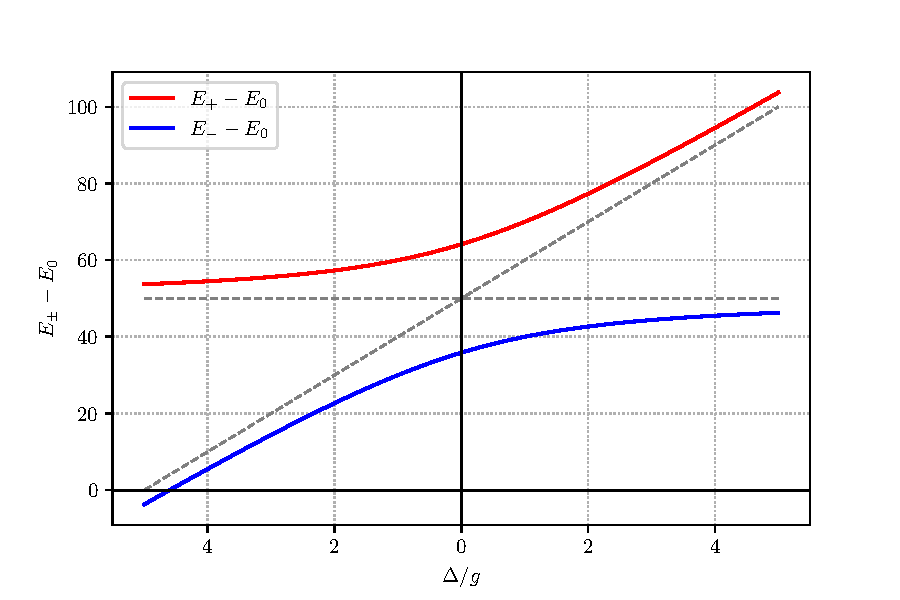
\includegraphics[scale=1]{images/graph.pdf}
    \caption{Differenza in energia dei dressed states con lo stato fondamentale in funzione del detuning. Si noti che la minima differenza di energia tra $E_+$ e $E_-$ si trova in corrispondenza di $\Delta = 0$, mentre la maggior differenza è data quando $\Delta$ diverge. L'asintoto orizzontale si trova in corrispondenza dei limiti: $\lim_{\Delta \to -\infty} (E_+-E_0) = \lim_{\Delta \to +\infty} (E_--E_0) = (n+1) \omega_c$. In questo caso si sono impostati i seguenti valori $\omega_c = 25$, $g=10$, $n=1$.}
    \label{fig:plot-dressed-states-detuning}
\end{figure}

\noindent Nel caso invece del qubit è possibile "giocare" con $g$, $n$ e $\Delta$ per osservare questo pattern di oscillazioni. Nella scorsa sezione abbiamo visto che in una situazione di risonanza esatta ($\Delta = 0$) vi era certezza che ad un certo punto il qubit avesse subito una transizione $\ket{0} \to \ket{1}$. Come vedremo tra poco, in altre situazioni può essere utile considerare il cosiddetto \textbf{regime dispersivo}, ossia $\Delta \neq 0$. Consideriamo l'energia dei \textbf{dressed states} come funzione del \textbf{detuning}: la differenza in energia con lo stato fondamentale non è altro che
\begin{equation*}
    E_\pm - E_0 = (n+1)\omega_c \pm \frac 12\sqrt{\Delta^2+4g^2(n+1)}+\frac \Delta 2 \, ;
\end{equation*}
se disegniamo un plot in funzione di $\frac{\Delta}{g}$ otteniamo la Figura \ref{fig:plot-dressed-states-detuning}. I due regimi particolarmente interessanti sono:
\begin{itemize}
    \item \textbf{Regime di risonanza}, quindi $\Delta = 0$ ($\omega_c=\omega_q$): in questo caso $\theta_n=\frac \pi 4$, per cui $\cos\theta_n=\sin\theta_n=\frac1{\sqrt2}$. Si dice che vi è un'\textbf{ibridizzazione massima} degli stati poiché
    \begin{equation*}
        \ket{n_\pm}= \frac{\ket{g,n+1}\pm\ket{e,n}}{\sqrt 2} \, ;
    \end{equation*}
    essi prendono il nome di \textbf{polarons}. La differenza in energia qui è la minima possibile e dipende da $n$:
    \begin{equation*}
        E_\pm = (n+1)\omega_c \pm g \sqrt{n+1} \, .
    \end{equation*}
    In generale è una situazione abbastanza simile alle oscillazioni di Rabi della Figura \ref{fig:Rabi}.
    
    \item \textbf{Regime dispersivo}, tale che $\Delta \gg g$: qui $\theta_n\ll 1$ e gli stati originali rimangono pressoché invariati a meno di piccole correzioni
    \begin{align*}
        \ket{n_-} &= \ket{g,n+1} + \dots \, , \\
        \ket{n_+} &= \ket{e,n} + \dots \, ;
    \end{align*}
    notiamo che questo comportamento è previsto dato che $\frac{\Delta}{g} \to \infty$ significa equivalentemente che $\Delta = \text{ cost}$ e $g \simeq 0$: siamo vicini al caso libero in cui il qubit e la radiazione e.m. sono quasi disaccoppiati. 

    \noindent Questo regime è interessante per diverse ragioni: ad esempio può essere utile tenere le piccole correzioni negli stati $\ket{n_+}$ e $\ket{n_-}$. Sviluppando la radice in $\frac{g^2}{\Delta^2}$ si ha
    \begin{align*}
        E_\pm &= (n+1)\omega_c \pm \frac 12 \sqrt{\Delta^2+4g^2(n+1)} \\
              &= (n+1)\omega_c \pm \frac{\Delta}{2} \sqrt{1+ \frac{4g^2}{\Delta^2}(n+1)} \\
              &= (n+1)\omega_c \pm \frac{\Delta}{2}\left(1+\frac{2g^2}{\Delta^2}(n+1)+\dots\right) \\
              &= (n+1)\omega_c \pm \left(\frac\Delta 2 +\frac{g^2}{\Delta}(n+1)+\dots\right) \, ;
    \end{align*}
    Osserviamo che possiamo ricavare le medesime energie dando una descrizione efficace del sistema con la seguente hamiltoniana
    \begin{equation}\label{eq:effective-hamiltonian}
        \hat H^{(2)}=\omega_c\left(\hat a^\dagger \hat a + \frac 12\right)-\frac{\omega_q}2\hat \sigma_3 - \frac{g^2}{\Delta}\left(\hat a^\dagger \hat a + \frac 12\right) \hat{\sigma}_3 + \frac{g^2}{2\Delta}\mathbb{I}_{2\times2} \, ,
    \end{equation}
    infatti
    \begin{align*}
        \hat H^{(2)}\ket{g, n+1} &= \omega_c\left(n+1+\frac 12\right)-\frac{\omega_q}{2}-\frac{g^2}{\Delta}(n+1) \\ 
        &= \omega_c(n+1)-\frac{\Delta}2 -\frac{g^2}\Delta(n+1) \equiv E_- \, , \\
        \hat H^{(2)}\ket{e,n} &= \omega_c\left(n+\frac 12\right) + \frac{\omega_q}2 + \frac{g^2}{\Delta}\left(n+ \frac 12\right) + \frac{g^2}{2\Delta} \\
        &= \omega_c(n+1)+\frac{\Delta}2 + \frac{g^2}\Delta(n+1) \equiv E_+ \, .
    \end{align*}
    Dunque possiamo dire che l'hamiltoniana efficace $\hat{H}^{(2)}$ descrive la fisica del sistema nel regime dispersivo. Sui libri si trovano spesso hamiltoniane più complicate: questa hamiltoniana è un esempio della cosiddetta \textbf{trasformazione di Schrieffer-Wolff}. Si tratta di scegliere l'operatore $\hat{U}$ della \eqref{S_eq_rotated_state} indipendente dal tempo e della forma 
    \begin{equation*}
        \hat U = e^{\hat{S}} \, , \quad \text{dove} \quad S^\dag = - S \, .
    \end{equation*}
    L'operatore $\hat{S}$ è scelto in maniera tale che si possa effettuare un'espansione in teoria delle perturbazioni su un opportuno parametro. Se l'hamiltoniana si scrive come $\hat{H} = \hat{H}_0 + \hat{H}_I$, allora si sceglie un $\hat{S}$ tale che $\comm{\hat{S}}{\hat{H}_0} = -\hat{H}_I$. Con un po' di algebra si dimostra che
    \begin{equation*}
        \hat{U} \hat{H} \hat{U}^\dag = \hat{H}_0 + \frac{1}{2} \comm{\hat{S}}{\hat{H}_I} + \order{S^3} \, .
    \end{equation*}
    Nel nostro caso, l'espressione di $\hat H^{(2)}$ si ottiene dall'espansione fino a $\order{g^2/\Delta^2}$ nel sistema ruotato dall'operatore
    \begin{equation*}
        \hat U = e^{-\frac{g}{\Delta}(\hat \sigma_+\hat a^\dagger - \hat \sigma_-\hat a)} \, .
    \end{equation*}
    
    Riscriviamo l'hamiltoniana \eqref{eq:effective-hamiltonian} senza i termini costanti:
    \begin{equation*}
        \hat H^{(2)} = \omega_c  \hat a^\dagger \hat a - \frac{\omega_q}2\hat \sigma_3 - \frac{g^2}{\Delta}\left(\hat a^\dagger \hat a + \frac 12\right) \hat{\sigma}_3 \, .
    \end{equation*}
    A seconda di ciò che si sta facendo è utile raggruppare gli operatori interni a questa espressione in due modi:
    
    \begin{itemize}
        \item Possiamo raggruppare scrivendo 
    \begin{equation*}
        \hat H^{(2)}= \left(\omega_c-\chi\hat \sigma_3\right)\hat a^\dagger \hat a-\frac{\tilde{\omega}_q}{2}\hat \sigma_3 \, ,
    \end{equation*}
    dove $\chi = g^2/\Delta$ e $\tilde{\omega}_q=\omega_q+g^2/\Delta$. È evidente che l'energia della cavità dipenderà da una frequenza che risulta shiftata di una costante $\chi$ dipendente dallo stato del qubit; similmente $\omega_q$ è ridefinito a seguito dell'interazione con il campo elettromagnetico (si parla infatti di \textbf{Lamb shift}, in onore dell'analogo in fisica atomica). Per tale ragione questa situazione può essere utilizzata per realizzare una \textbf{quantum nondemolition measurement}: possiamo stabilire lo stato in cui si trova il qubit misurando la frequenza della cavità! Si noti che questo non viola le leggi della QM.
    
    \item Un modo equivalente è quello di raggruppare tutte le matrici $\hat{\sigma_3}$ scrivendo
    \begin{equation*}
        \hat H^{(2)}= \omega_c\hat a^\dagger \hat a - \frac{\hat \sigma_3}{2}\left(\omega_q + \frac{g^2}{\Delta}+\frac{2g^2}{\Delta}\hat a^\dagger \hat a \right) \, ;
    \end{equation*}
    in questa visione la frequenza del qubit è ridefinita a seguito di due fattori: il Lamb shift (secondo termine della parentesi) e il cosiddetto \textbf{AC - Stark Effect} (ultimo termine), il quale indica il numero di fotoni che creano rumore nella frequenza dei qubit; quindi in questo caso anche il numero di fotoni influenza la frequenza del qubit. 
    \end{itemize}
\end{itemize}

\subsection{Operazioni su 2 qubit}
Il regime dispersivo nel sistema qubit-cavità può essere utilizzato per codificare delle operazioni (gate) che coinvolgono due qubit. Ricordiamo che nella sezione precedente abbiamo visto che le operazioni sui \textbf{singoli} qubit sono realizzate abbastanza semplicemente per mezzo delle oscillazioni di Rabi. Qui il trucco è quello introdurre uno stato addizionale, che chiamiamo $\ket{\gamma}$, al fuori della cavità risonante (in cui sono presenti gli stati $\ket{g}$ e $\ket{e}$ che interagiscono con i fotoni):
\begin{center}
    \mbox{
        \Qcircuit @C=1em @R=2em {
            \lstick{\ket{e}} & \qw & \qw & \qw \\
            \lstick{\ket{g}} & \qw & \qw & \qw
        }
    }
    \raisebox{-1em}{\mbox{
        \Qcircuit @C=1em @R=2em {
            & \qw & \qw & \qw & \rstick{\ket{\gamma}} \\
        }
    }}
\end{center}
Precisiamo che $\ket{e}$ e $\ket{g}$ sono accoppiati con la cavità, mentre $\ket \gamma$ è disaccoppiato dal sistema qubit-cavità. L'idea è quella di codificare un qubit con gli stati $( \ket g, \ket \gamma)$ e uno con gli stati $(\ket 0, \ket 1)$ dei fotoni, cosicché lo spazio di Hilbert totale contenga gli stati seguenti
\begin{equation*}
    \mathcal{H}=\left\{\ket{\gamma 0}, \ket{\gamma 1}, \ket{g0}, \ket{g1}\right\} \, .
\end{equation*}
L'interazione sarà descritta dall'hamiltoniana \eqref{eq:effective-hamiltonian}: lo stato $\ket{e}$ è irrilevante in questa descrizione, mentre l'accoppiamento qubit-cavità è dato dagli ultimi due termini interagenti (quelli con $g$). Consideriamo l'evoluzione temporale del sistema del qubit: gli operatori $\hat{\sigma}_3$ e $\mathbb{I}$ agiscono solamente su $\ket{e}$ e $\ket{g}$ perché $\ket{\gamma}$ è disaccoppiato. Per tale motivo, dal momento che $\hat \sigma_3\ket{\gamma}=\mathbb{I}\ket{\gamma}=0$ e $\hat \sigma_3\ket{g}=\ket{g}$, la parte interagente di $\hat{H}^{(2)}$ agisce come
\begin{equation*}
    e^{-i \hat{H}_{I}^{(2)} t}=e^{i\frac{g^2}{\Delta}\hat a^\dagger \hat a \hat \sigma_3 t + i\frac{g^2}{2\Delta}(\hat \sigma_3 - \mathbb{I}_{2\times2})t}=\begin{pmatrix}
        1 & & & \\
        & 1 & & \\
        & & 1 & \\
        & & & e^{i\frac{g^2}{\Delta}t}
    \end{pmatrix}
    \begin{matrix}
        \ket{\gamma 0} \\ \ket{\gamma 1} \\ \ket{g 0} \\ \ket{g1}
    \end{matrix} \, .
\end{equation*}
(come in precedenza sono scritti gli stati sulla destra per ricordare l'origine degli elementi di matrice). Il gate risultante è detto \textbf{QPG}, ossia \textbf{Quantum Phase Gate}, poiché è della forma
\begin{equation*}
    Q_\eta = \begin{pmatrix}
        1 & & & \\
        & 1 & & \\
        & & 1 & \\
        & & & e^{i\eta}
    \end{pmatrix} \, .
\end{equation*}
Questa tipologia di gate include il caso $\eta = \pi$, ovvero 
\begin{equation*}
    Q_\pi = \begin{pmatrix}
        1 & & & \\
        & 1 & & \\
        & & 1 & \\
        & & & -1
    \end{pmatrix} \, ;
\end{equation*}
il gate precedente potrebbe sembrare banale ma non lo è perché, usando operazioni a singolo gate su $\ket{\gamma}$ e $\ket{g}$, esso può essere convertito in un \texttt{CZ-gate} (Controlled-$Z$)
\begin{center}
    \mbox{
        \Qcircuit @C=1em @R=1em {
            & \qw & \ctrl{1} & \qw & \qw & \\
            & \qw & \gate{Z} & \qw & \qw &
        }
    }
\end{center}
ma sappiamo che quest'ultimo è legato al \texttt{CNOT-gate} attraverso l'applicazione di due \texttt{H-gate}

\begin{center}
    \mbox{
        \Qcircuit @C=1em @R=1.2em {
            & \qw & \ctrl{1} & \qw & \qw & \\
            & \qw & \targ & \qw & \qw &
        }
    }
    \raisebox{-1em}{=}
    \mbox{
        \Qcircuit @C=1em @R=1em {
            & \qw & \ctrl{1} & \qw & \qw & \\
            & \gate{H} & \gate{Z} & \gate{H} & \qw &
        }
    }
\end{center}
Questo significa che con delle singole operazioni possiamo trasformare un QPG in un \texttt{CNOT-gate}, che sappiamo molto bene che agisce su due qubit contemporaneamente. 

\noindent Cosa succede invece ai termini non interagenti in \eqref{eq:effective-hamiltonian}? Anche loro permettono di implementare delle trasformazioni sui qubit: l'evoluzione temporale dell'hamiltoniana libera è disaccoppiata poiché $\hat{H}^{(2)}_0$ è somma delle hamiltoniane del qubit e della cavità. Perciò questa evoluzione può sempre essere fattorizzata come
\begin{equation*}
    e^{-i\omega_c\left(\hat a^\dagger \hat a + \frac 12\right)t + i\frac{\omega_q}{2}\hat \sigma_3t} = e^{-i\omega_c\left(\hat a^\dagger \hat a + \frac 12\right)t}e^{i\frac{\omega_q}{2}\hat \sigma_3t}=
    e^{-i\frac{\omega_c}{2}t}
    \underbrace{\begin{pmatrix}
        1 & 0\\
        0 & e^{i\frac{\omega_q}{2}t}
    \end{pmatrix}
    }_{\{\ket \gamma, \ket g\}}
    \otimes
    \underbrace{
    \begin{pmatrix}
        1 & 0\\
        0 & e^{-i\omega_c t}
    \end{pmatrix}
    }_{\{\ket 0, \ket 1\}} \, .
\end{equation*}
Questo è un fatto generale: l'evoluzione libera descrive sempre l'evoluzione del singolo qubit perché $\hat{H}^{(2)}_0$ è fattorizzata. 

\noindent Nelle prossime sezioni vedremo alcuni esempi espliciti, come qubit superconduttivi e trappole ioniche, che metteranno in pratica i concetti che abbiamo studiato nel corso delle ultime due sezioni. In generale non è così difficile creare i gate, ma la difficoltà spesso risiede nel controllarli; spesso le idee funzionanti sono frutto di intuizioni creative e geniali legate al trovare la corretta evoluzione temporale del sistema. 